\newpage
\section{Organizacja projektu}

\subsection{Struktura organizacyjna}
Struktura zespołu projektowego jest przedstawiona
na~rys.~\ref{fig:organizacja:hierarchia}
na~stronie~\pageref{fig:organizacja:hierarchia}.
\begin{figure}[h!]
    \centering
    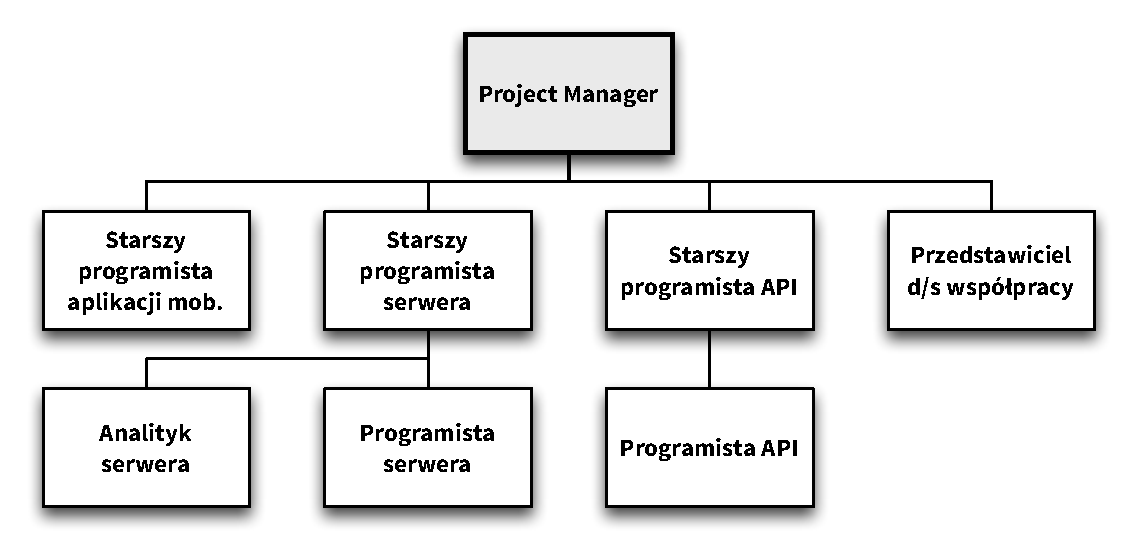
\includegraphics[width=0.9\textwidth]{./figury/organizacja-projektu/hierarchia}
    \caption{Schemat struktury organizacyjnej zespołu projektowego.}
    \label{fig:organizacja:hierarchia}
\end{figure}

\subsection{Plan zatrudnienia}
Planowane jest rozdzielenie ról według schematu z rys.~\ref{fig:organizacja:plan_zatrudnienia}.
na~stronie~\pageref{fig:organizacja:plan_zatrudnienia}.
\begin{figure}[h!]
    \centering
    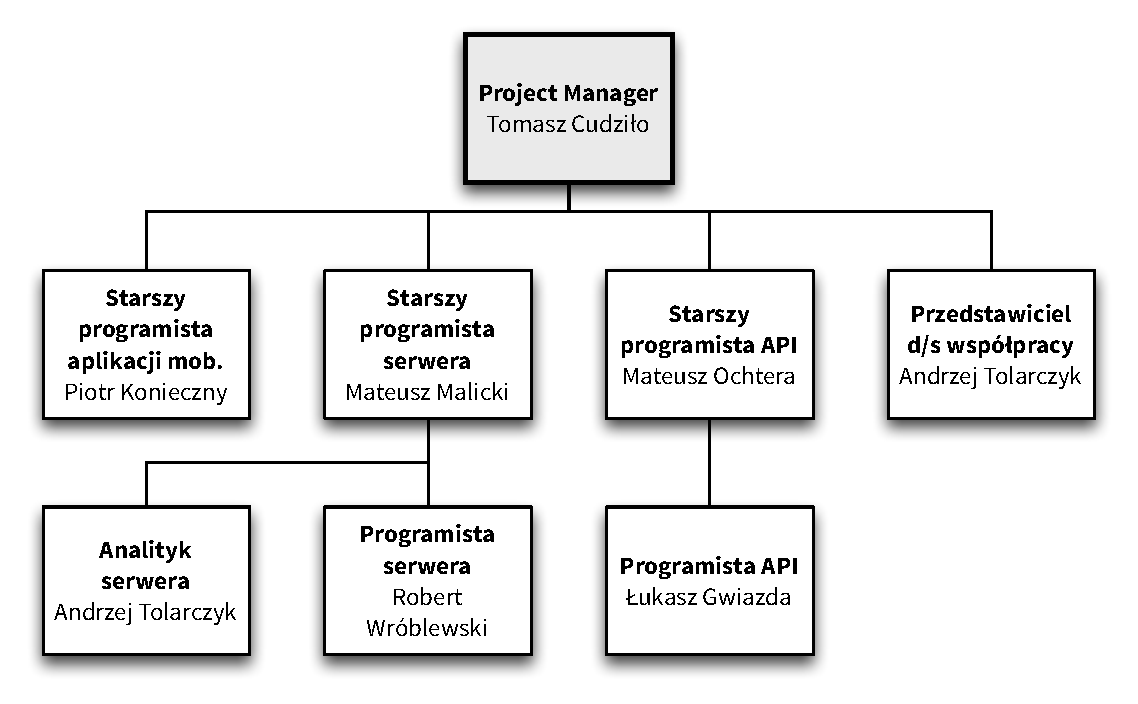
\includegraphics[width=0.9\textwidth]{./figury/organizacja-projektu/plan-zatrudnienia}
    \caption{Schemat przydziału ról w zespole projektowym.}
    \label{fig:organizacja:plan_zatrudnienia}
\end{figure}

\subsection{Granice organizacyjne}
Zespół projektowy \emph{Concerto} jest niezależną jednostką. Nawiązywanie
współpracy wymaga kontaktu z przedstawicielem biznesowym organizatora wydarzeń
kulturalnych. Po nawiązaniu współpracy, w wyjątkowych sytuacjach, komunikacja
odbywa się z działem IT oraz osobą odpowiedzialną za przeprowadzane akcje
reklamowe -- przedstawicieli wyznaczonych ze strony organizatora wydarzeń.
Produkt projektu -- API stanowi podstawowy kanał komunikacyjny, dla
standardowych zdarzeń.

\subsection{Podział odpowiedzialności}
Macierze odpowiedzialności za kolejne grupy zadań przewidzianych w pracach nad
projektem są załączone zaczynając od~strony~\pageref{fig:organizacja:macierz}.

Zadania organizacyjne, zarządzania projektem i reprezentowania zespołu
projektowego, jeżeli nie uwzględnione w macierzach odpowiedzialności, są
odpowiedzialnością Project Managera.

\begin{figure}[p]
    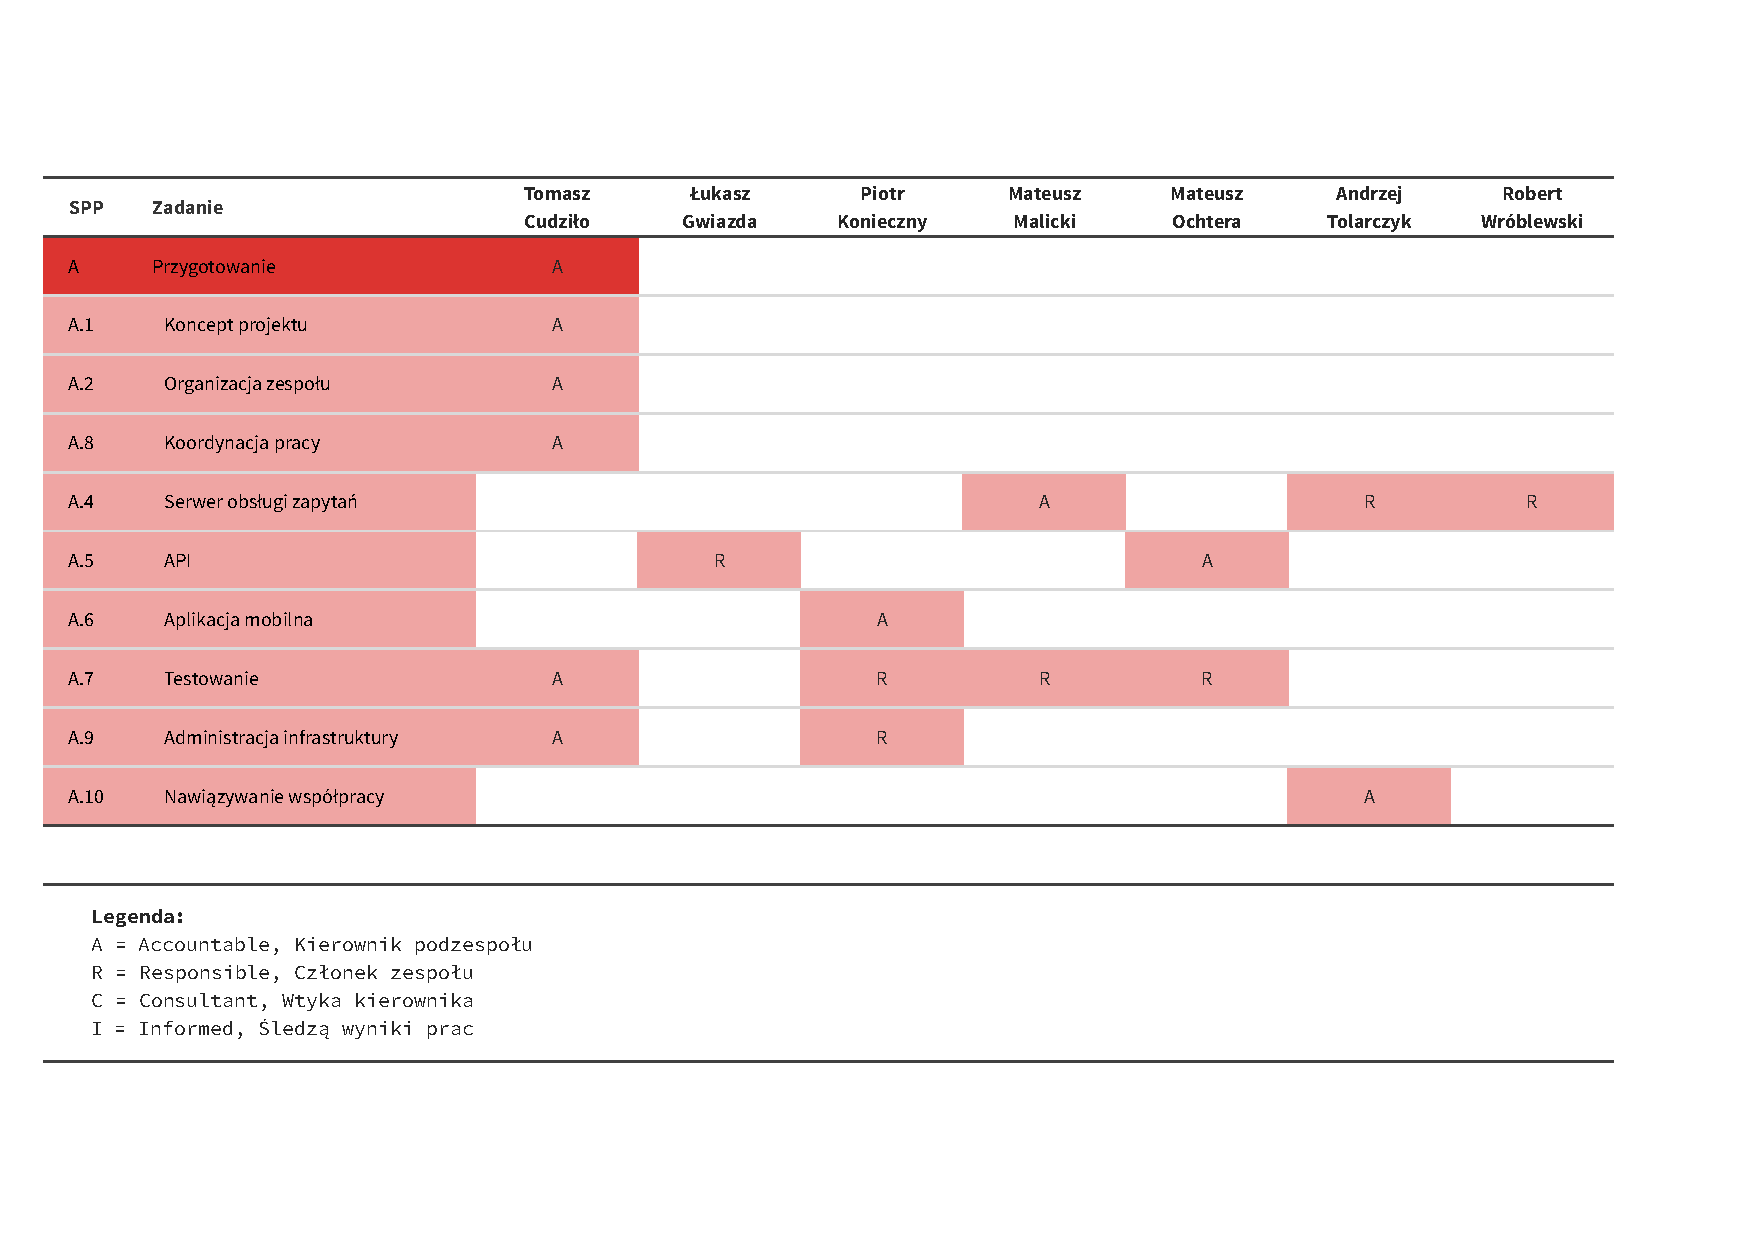
\includegraphics[angle=270, trim=1cm 1cm 1cm 1cm, width=\textwidth]{./figury/organizacja-projektu/macierz-odpowiedzialnosci-A-przygotowanie}
    \caption{Macierz odpowiedzialności za zadania w iteracji \emph{Przygotowanie}.}
    \label{fig:organizacja:macierz}
\end{figure}

\begin{figure}[p]
    \ContinuedFloat
    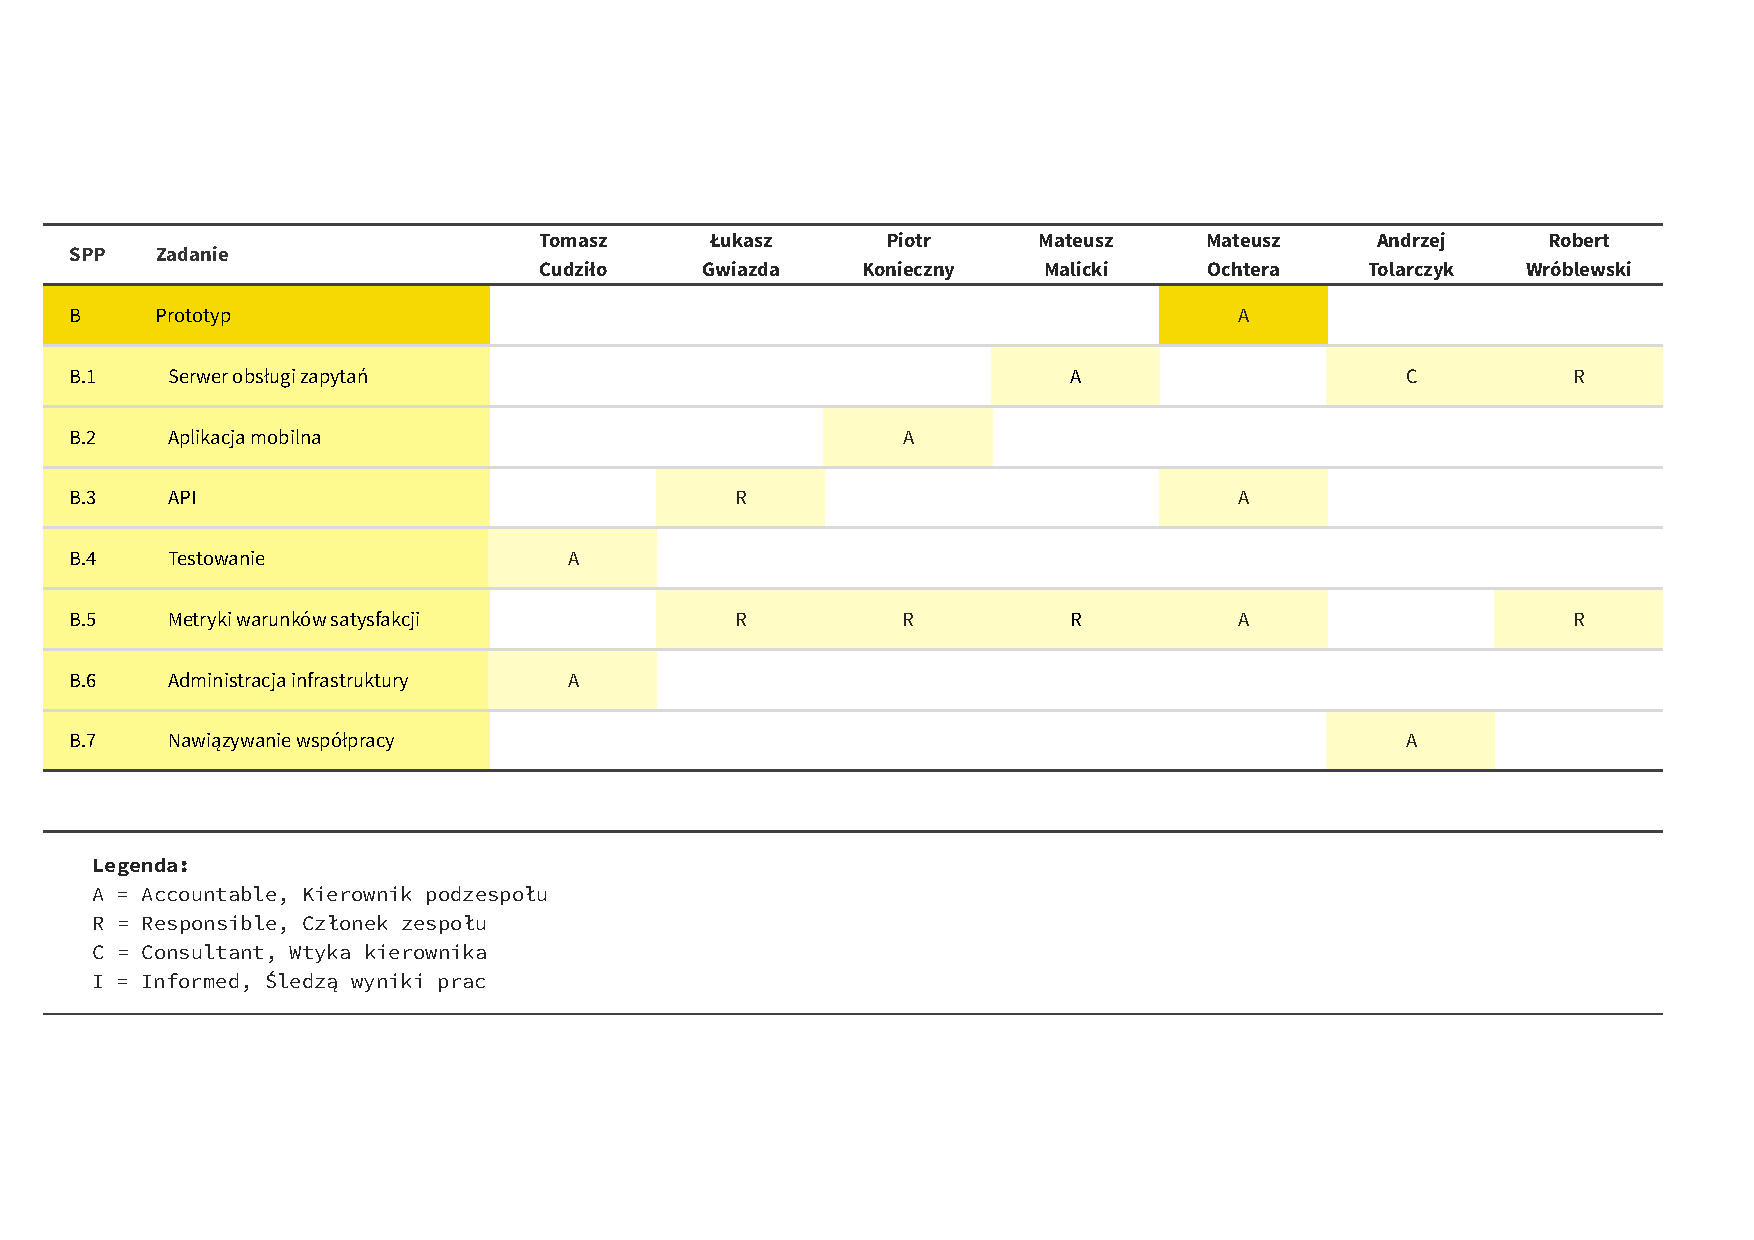
\includegraphics[angle=270, trim=1cm 1cm 1cm 1cm, width=\textwidth]{./figury/organizacja-projektu/macierz-odpowiedzialnosci-B-prototyp}
    \caption[]{Macierz odpowiedzialności za zadania iteracji \emph{Prototyp}.}
\end{figure}

\begin{figure}[p]
    \ContinuedFloat
    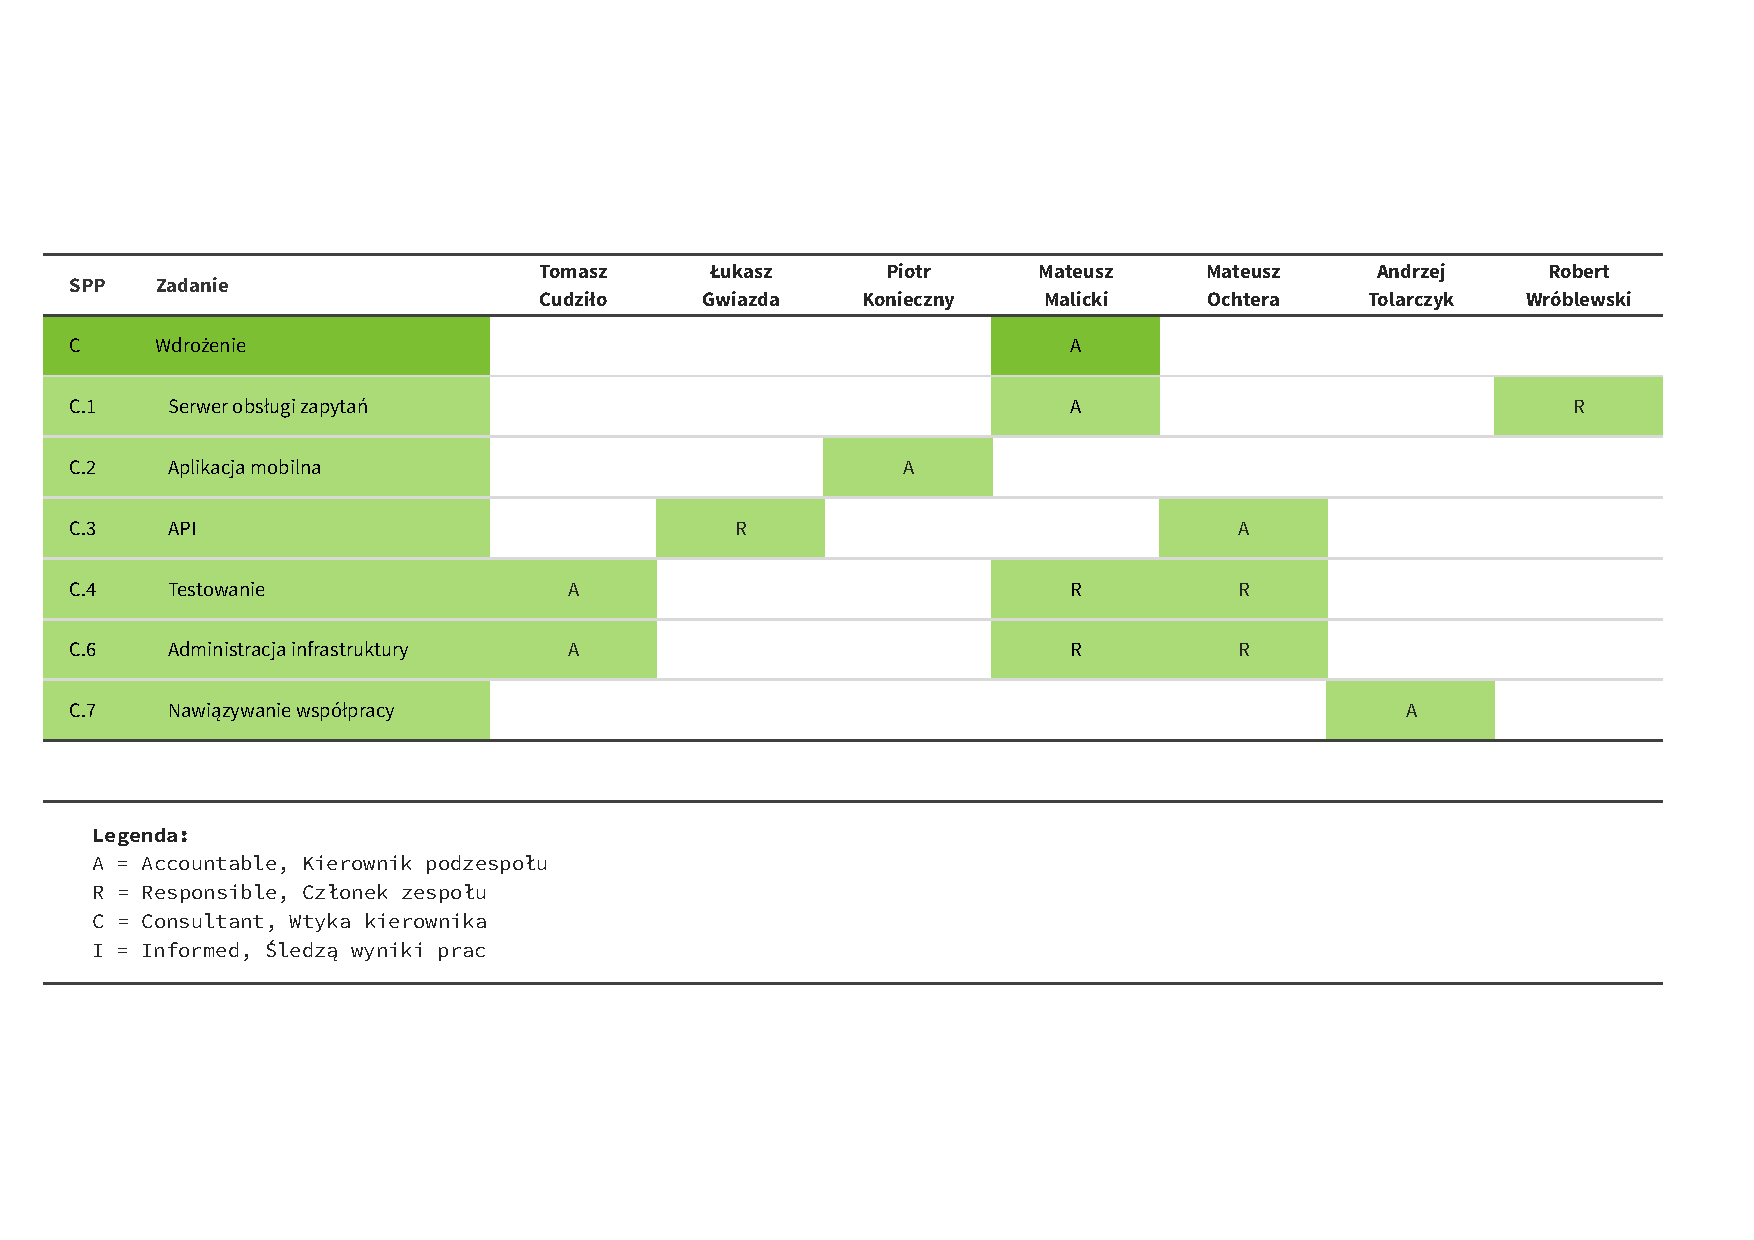
\includegraphics[angle=270, trim=1cm 1cm 1cm 1cm, width=\textwidth]{./figury/organizacja-projektu/macierz-odpowiedzialnosci-C-wdrozenie}
    \caption[]{Macierz odpowiedzialności za zadania iteracji \emph{Wdrożenie}.}
\end{figure}
